\section{European Social Survey}\label{sec:ess}

\subsection{What the data can and cannot show}

The latent $\theta_{K+1}$ is unobserved. \textbf{No coverage is claimed or
computed here}, and a held-out region's direct estimate is not a substitute for
the latent value: treating it as one would measure the uncorrected anchor. What
real data can show is which inputs each construction needs, how far the intervals
differ on the same data, and which assumptions the data support.

\subsection{Design}

Rounds 9--11, 127{,}286 respondents, 75 country-rounds, 825 region-rounds,
retrieved through the portal API so that the analysis reproduces from source for
any user with an End User Licence. Everything was fixed before any estimate was
computed: the target is a single CDF point $F_{cr}(t_0)$ with $t_0$ set by rule
(one below the scale midpoint); three items chosen in advance for differing
between-region heterogeneity; the structure variable $x_{cr}$ is the region's
sampled PSU count, carried over unchanged from the simulations; one budget for
every arm; the comparator's split fixed rather than scanned. Regions with fewer
than two design degrees of freedom (18 of 825) are excluded and counted; regions
with a zero variance estimate (13, 39, 55 by item) receive no shrinkage, which is
conservative.

\subsection{The score and its variance must match}

The score is $Y_{cr}=\Fhat_{cr}-\Fhat_c$, a deviation from an \emph{estimated}
country centre. Its design variance is not that of $\Fhat_{cr}$: it is that of the
difference, and we compute it from the Taylor linearisation
\[
u_i=\frac{w_i\mathbf 1\{i\in r\}(z_i-\Fhat_{cr})}{W_r}-\frac{w_i(z_i-\Fhat_c)}{W_c}
\]
aggregated to PSU totals over the whole country-round. \textbf{This is not a
technicality.} With the wrong variance the fitted structure exponent has median
$0.53$ and its confidence set contains the elementary value $\gamma=1$
($D\propto1/n$) in \emph{none} of 45 configurations, including one implausible
negative estimate; with the right one the median is $1.14$ and the set contains
$\gamma=1$ in 17 of 45.

\subsection{What the arms do on the same data}

\begin{center}
\begin{tabular}{lcc}
\toprule
comparison & range over 45 configurations & \\
\midrule
proposed / normal-theory comparator & 0.729--1.014 & narrower in \textbf{44 of 45}, median 0.821\\
proposed / structure-free & 0.459--1.034 & narrower in 43 of 45, median 0.830\\
proposed / uncorrected & 0.422--0.867 & median 0.730\\
\bottomrule
\end{tabular}
\end{center}

\begin{figure}[t]
\centering
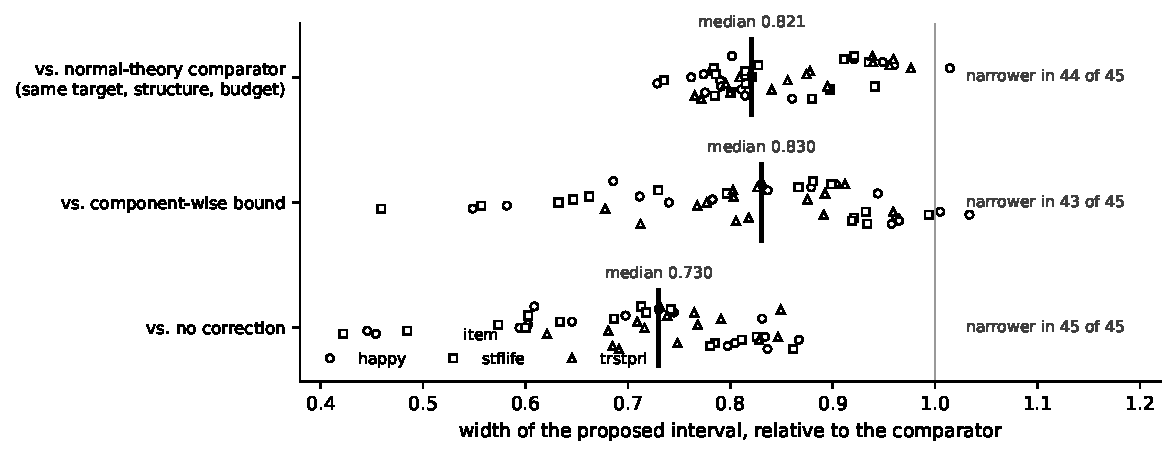
\includegraphics[width=\textwidth]{figures/fig2_ess_widths}
\caption{Width of the proposed interval relative to each comparator, over the 45
item-by-round-by-country configurations of European Social Survey rounds 9--11.
Bars are medians. All three comparisons use the variance of the centred score
(Section~\ref{sec:ess}); with the uncorrected variance the middle comparison
moves to a median of $0.992$. \textbf{No coverage is claimed}: the latent target
is unobserved.}
\label{fig:ess}
\end{figure}

The comparison against a comparator sharing the target reproduces the simulation
on real data---median 0.821 against a simulated 13.9--22.2\% reduction---and is
the robust one, because both arms are built on the same variance. Realised design
shares are $\widehat\rho^2\in[0.22,0.61]$: the regime the correction is for.

\subsection{Which assumptions the data support}

The pivot needs normality of the standardised regional deviations. Skewness and
excess kurtosis are $-0.47$ to $0.62$ and $0.3$ to $4.4$ for the first item, and
reach $2.30$ and $12.6$, and $2.81$ and $17.6$, for the other two.
\textbf{The condition is reasonably supported for one item of the three and
clearly not for the others}, and we report that with their results.

The structure model explains 0.09 to 0.23 of $\log\Dhat$ once the right variance
is used---moderately at best.

\paragraph{This is not the quantity that separated the two columns of
Section~\ref{sec:simulation}, and the two must not be compared.} There the
structure $R^2$ was computed against the \emph{true} design variances, which a
simulation supplies and a survey does not; here it is computed against estimated
ones, and estimation noise in $\log\Dhat$ depresses it by an amount we cannot
remove. A reader should therefore not conclude from $0.09$--$0.23$ that these
data sit in the regime where the procedure lost containment---nor that they sit
in the safe one. The honest statement is that the diagnostic available on real
data does not identify which column a real survey belongs to, and supplying that
mapping would require knowing the design variances one is trying to estimate. An analyst can compute that quantity, and across
these 45 configurations it is associated with whether using the structure pays
(correlation $-0.30$). \textbf{We report this as an observable exploratory
diagnostic and not as a criterion}: both quantities are built from the same
variance estimates so part of any association is arithmetic, and a good structure
fit does not imply coverage, which is not measured here.

\subsection{The approximation this analysis rests on}

Correcting the variance does not restore exchangeability. A common estimated
centre makes the scores dependent, and we measure it: the mean within-country
correlation among distinct regions is $-0.232$, $-0.116$, $-0.046$, $-0.029$ for
country-rounds with at most 5, 6--10, 11--20 and more than 20 regions---almost
exactly $-1/(n_r-1)$, the classical dependence of deviations from a common mean.
It is negative, hence the benign direction for a maximum-based rank statistic,
and it shrinks with the number of regions, but it is not zero.

\begin{quote}
\textbf{Status of this analysis.} An application of the procedure under a stated
approximation: the centre is estimated rather than known, and the scores carry a
measured dependence of about $-1/(n_r-1)$. \textbf{The guarantee of
Section~\ref{sec:method} is not attached to it.}
\end{quote}
